\documentclass[aspectratio=169, 11pt]{beamer}

% ==============================================================================
% CONFIGURAÇÃO DE CORES (Tons Pastéis & Light Mode)
% ==============================================================================
\usepackage{xcolor}

% Definição de Tons Pastéis
\definecolor{PastelBlue}{RGB}{173, 216, 230}
\definecolor{PastelGreen}{RGB}{152, 251, 152}
\definecolor{PastelPurple}{RGB}{221, 160, 221}
\definecolor{PastelYellow}{RGB}{253, 253, 150}
\definecolor{DarkGray}{RGB}{60, 60, 60}
\definecolor{SoftGray}{RGB}{245, 245, 245}

% Configuração do Tema Beamer
\mode<presentation> {
    \usetheme{Boadilla}
    \usecolortheme{default}
    
    % Aplicando as cores pastéis na estrutura
    \setbeamercolor{palette primary}{bg=PastelBlue, fg=DarkGray}
    \setbeamercolor{palette secondary}{bg=PastelGreen, fg=DarkGray}
    \setbeamercolor{palette tertiary}{bg=PastelPurple, fg=DarkGray}
    \setbeamercolor{palette quaternary}{bg=PastelYellow, fg=DarkGray}
    
    \setbeamercolor{structure}{fg=DarkGray}
    \setbeamercolor{background canvas}{bg=SoftGray}
    \setbeamercolor{normal text}{fg=DarkGray}
    
    \setbeamercolor{title}{bg=PastelBlue, fg=DarkGray}
    \setbeamercolor{frametitle}{bg=PastelBlue, fg=DarkGray}
    \setbeamercolor{block title}{bg=PastelPurple, fg=DarkGray}
    \setbeamercolor{block body}{bg=white, fg=DarkGray}
    
    % Desativar símbolos de navegação
    \setbeamertemplate{navigation symbols}{}
}

% ==============================================================================
% PACOTES E IDIOMA
% ==============================================================================
\usepackage[utf8]{inputenc}
\usepackage[brazil]{babel}
\usepackage{graphicx}
\usepackage{booktabs}
\usepackage{amsmath}
\usepackage{algorithm}
\usepackage{algpseudocode}

% ==============================================================================
% DADOS DA APRESENTAÇÃO
% ==============================================================================
\title[SSSP Algoritmos]{Análise Comparativa SSSP: \\ Dijkstra, Bellman-Ford e BMSSP}
\subtitle{Quebrando a Barreira de Ordenação em Grafos}
\author[Equipe SSSP]{
  \textbf{Dupla A}: Algoritmos | \textbf{Dupla B}: Engenharia | \textbf{Dupla C}: Documentação
}
\institute[UNIFAL-MG]{Universidade Federal de Alfenas -- UNIFAL-MG}
\date{\today}

% ==============================================================================
% INÍCIO DO DOCUMENTO
% ==============================================================================
\begin{document}

\begin{frame}
    \titlepage
\end{frame}

\begin{frame}{Sumário}
    \tableofcontents
\end{frame}

% ==============================================================================
\section{Introdução e Objetivos}
% ==============================================================================
\begin{frame}{Introdução e Objetivos}
    \begin{block}{O Problema (SSSP)}
        Dada uma origem única, determinar a distância mínima para todos os outros vértices do grafo. Algoritmos clássicos enfrentam uma \textbf{barreira de ordenação} de vértices.
    \end{block}
    
    \vspace{0.5cm}
    \textbf{Objetivos deste Projeto (TP 03):}
    \begin{itemize}
        \item Implementar o Dijkstra com \textit{Min-Heap} iterativo.
        \item Implementar o \textit{Bellman-Ford} como \textit{baseline} incondicional.
        \item Reproduzir e avaliar a complexidade $O(m \log^{2/3} n)$ do algoritmo recursivo Bounded Multi-Source Shortest Path (\textbf{BMSSP}) de \textit{Duan et al. (2023)}.
        \item Criar um pipeline de coleta empírica $N$ vs. Tempo de Execução.
    \end{itemize}
\end{frame}

% ==============================================================================
\section{Estrutura Matricial da Equipe}
% ==============================================================================
\begin{frame}{Governança e Estrutura da Equipe (Matricial)}
    Para evitar silos de desenvolvimento, 6 membros atuarão em 3 duplas (\textbf{Cross-Functional}):
    
    \vspace{0.3cm}
    \begin{columns}
        \column{0.33\textwidth}
        \begin{block}{Dupla A (Core C)}
            Foco: Corretude do Dijkstra e BMSSP. \\
            Revisão cruzada pela Dupla B.
        \end{block}
        
        \column{0.33\textwidth}
        \begin{block}{Dupla B (Python Pipeline)}
            Foco: Gerador Erdos-Renyi e Orquestração (\texttt{make}). \\
            Revisão cruzada pela Dupla C.
        \end{block}
        
        \column{0.33\textwidth}
        \begin{block}{Dupla C (LaTeX \& Relatoria)}
            Foco: Artigo final, Beamer e conformidade bibliográfica. \\
            Revisão cruzada pela Dupla A.
        \end{block}
    \end{columns}
    
    \vspace{0.5cm}
    \textbf{Vantagem de Ponta a Ponta:} Qualquer membro consegue simular e analisar todo o repositório em sua máquina através do comando único \texttt{make all}, trocando de papéis dinamicamente.
\end{frame}

% ==============================================================================
\section{Fundamentação Teórica: Algoritmo BMSSP}
% ==============================================================================
\begin{frame}{O Algoritmo BMSSP (Duan et al., 2023)}
    A referência do algoritmo BMSSP quebra a barreira de ordenação (Dijkstra restrito a $O(m \log n)$) através de particionamento e recursividade.
    
    \vspace{0.2cm}
    \begin{itemize}
        \item \textbf{Amostragem Estocástica:} O conjunto ativo $S$ é comprimido em um menor conjunto de pivôs $P$ via \texttt{FindPivots}, que explora as bordas.
        \item \textbf{Limites Superiores ($B$):} O algoritmo estipula bounds limitantes e atende a chamadas menores recursivas (nível $l$ da árvore decresce até o caso base onde atua o Dijkstra simples).
        \item \textbf{Custo Analítico:} O particionamento em pivôs e limites evita varrer a fila inteira para achar o mínimo absoluto. Resulta em tempo dominante dominado pela profundidade $l = \lceil \frac{\log n}{t} \rceil$, chegando a \textbf{$O(m \log^{2/3} n)$}.
    \end{itemize}
\end{frame}

\begin{frame}[fragile]{Pseudocódigo: BMSSP (Duan et al.)}
    \begin{algorithm}[H]
        \caption{BMSSP Simplificado}
        \small
        \begin{algorithmic}[1]
            \Procedure{BMSSP}{$G, S, B, l$}
                \If{$l == 0$ ou $S = \emptyset$} \Comment{Caso base: Alcançou o fundo da recursão}
                    \State Dijkstra em $G$ com origens $S$ até a distância limite $B$
                \Else
                    \State $k \gets \lfloor \log^{1/3} n \rfloor$ \Comment{Fator de compressão}
                    \State $P \gets \Call{FindPivots}{S, k}$ \Comment{Amostra $\approx |S|/k$ pivôs}
                    \State \Call{BMSSP}{$G, P, B, l - 1$} \Comment{Busca rápida guiada por pivôs}
                    \State \Call{BMSSP}{$G, S, B, l - 1$} \Comment{Busca refinada com conjunto completo}
                \EndIf
            \EndProcedure
        \end{algorithmic}
    \end{algorithm}
    \vspace{0.2cm}
    \small \textbf{Impacto:} Ao focar em $P$, a técnica relaxa iterativamente os bounds ($B$) da árvore de busca, quebrando o gargalo teórico de $O(m \log n)$ inerente à ordenação irrestrita.
\end{frame}
% ==============================================================================
\section{Implementação Computacional}
% ==============================================================================
\begin{frame}{Automação da Instanciação e Profilometria}
    O desenvolvimento em C foi conectado a scripts em Python para uma análise empírica massiva:
    
    \begin{block}{Execução Pipeline (Zero-Noise)}
        \begin{enumerate}
            \item \textbf{Gerador de Instâncias:} A partir do \texttt{networkx}, grafos variados ($N \in [50, 1000]$) são passados pela entrada padrão ao binário C.
            \item \textbf{Execução e Extração:} O tempo processual (profilometria via \texttt{clock()}) é coletado para os 3 algoritmos SSSP concorrentes.
            \item \textbf{Renderização Gráfica:} Um gráfico é embutido dinamicamente no relatório SBC.
        \end{enumerate}
    \end{block}
    
    A implementação precisou domar as estruturas de \textbf{ponteiros, Min-Heaps e memória} do BMSSP, garantindo que os subconjuntos de pivôs e matrizes de adjacência coubessem na memória de cache L2/L3.
\end{frame}

\begin{frame}{Resultados Empíricos e Gráficos}
    \begin{center}
        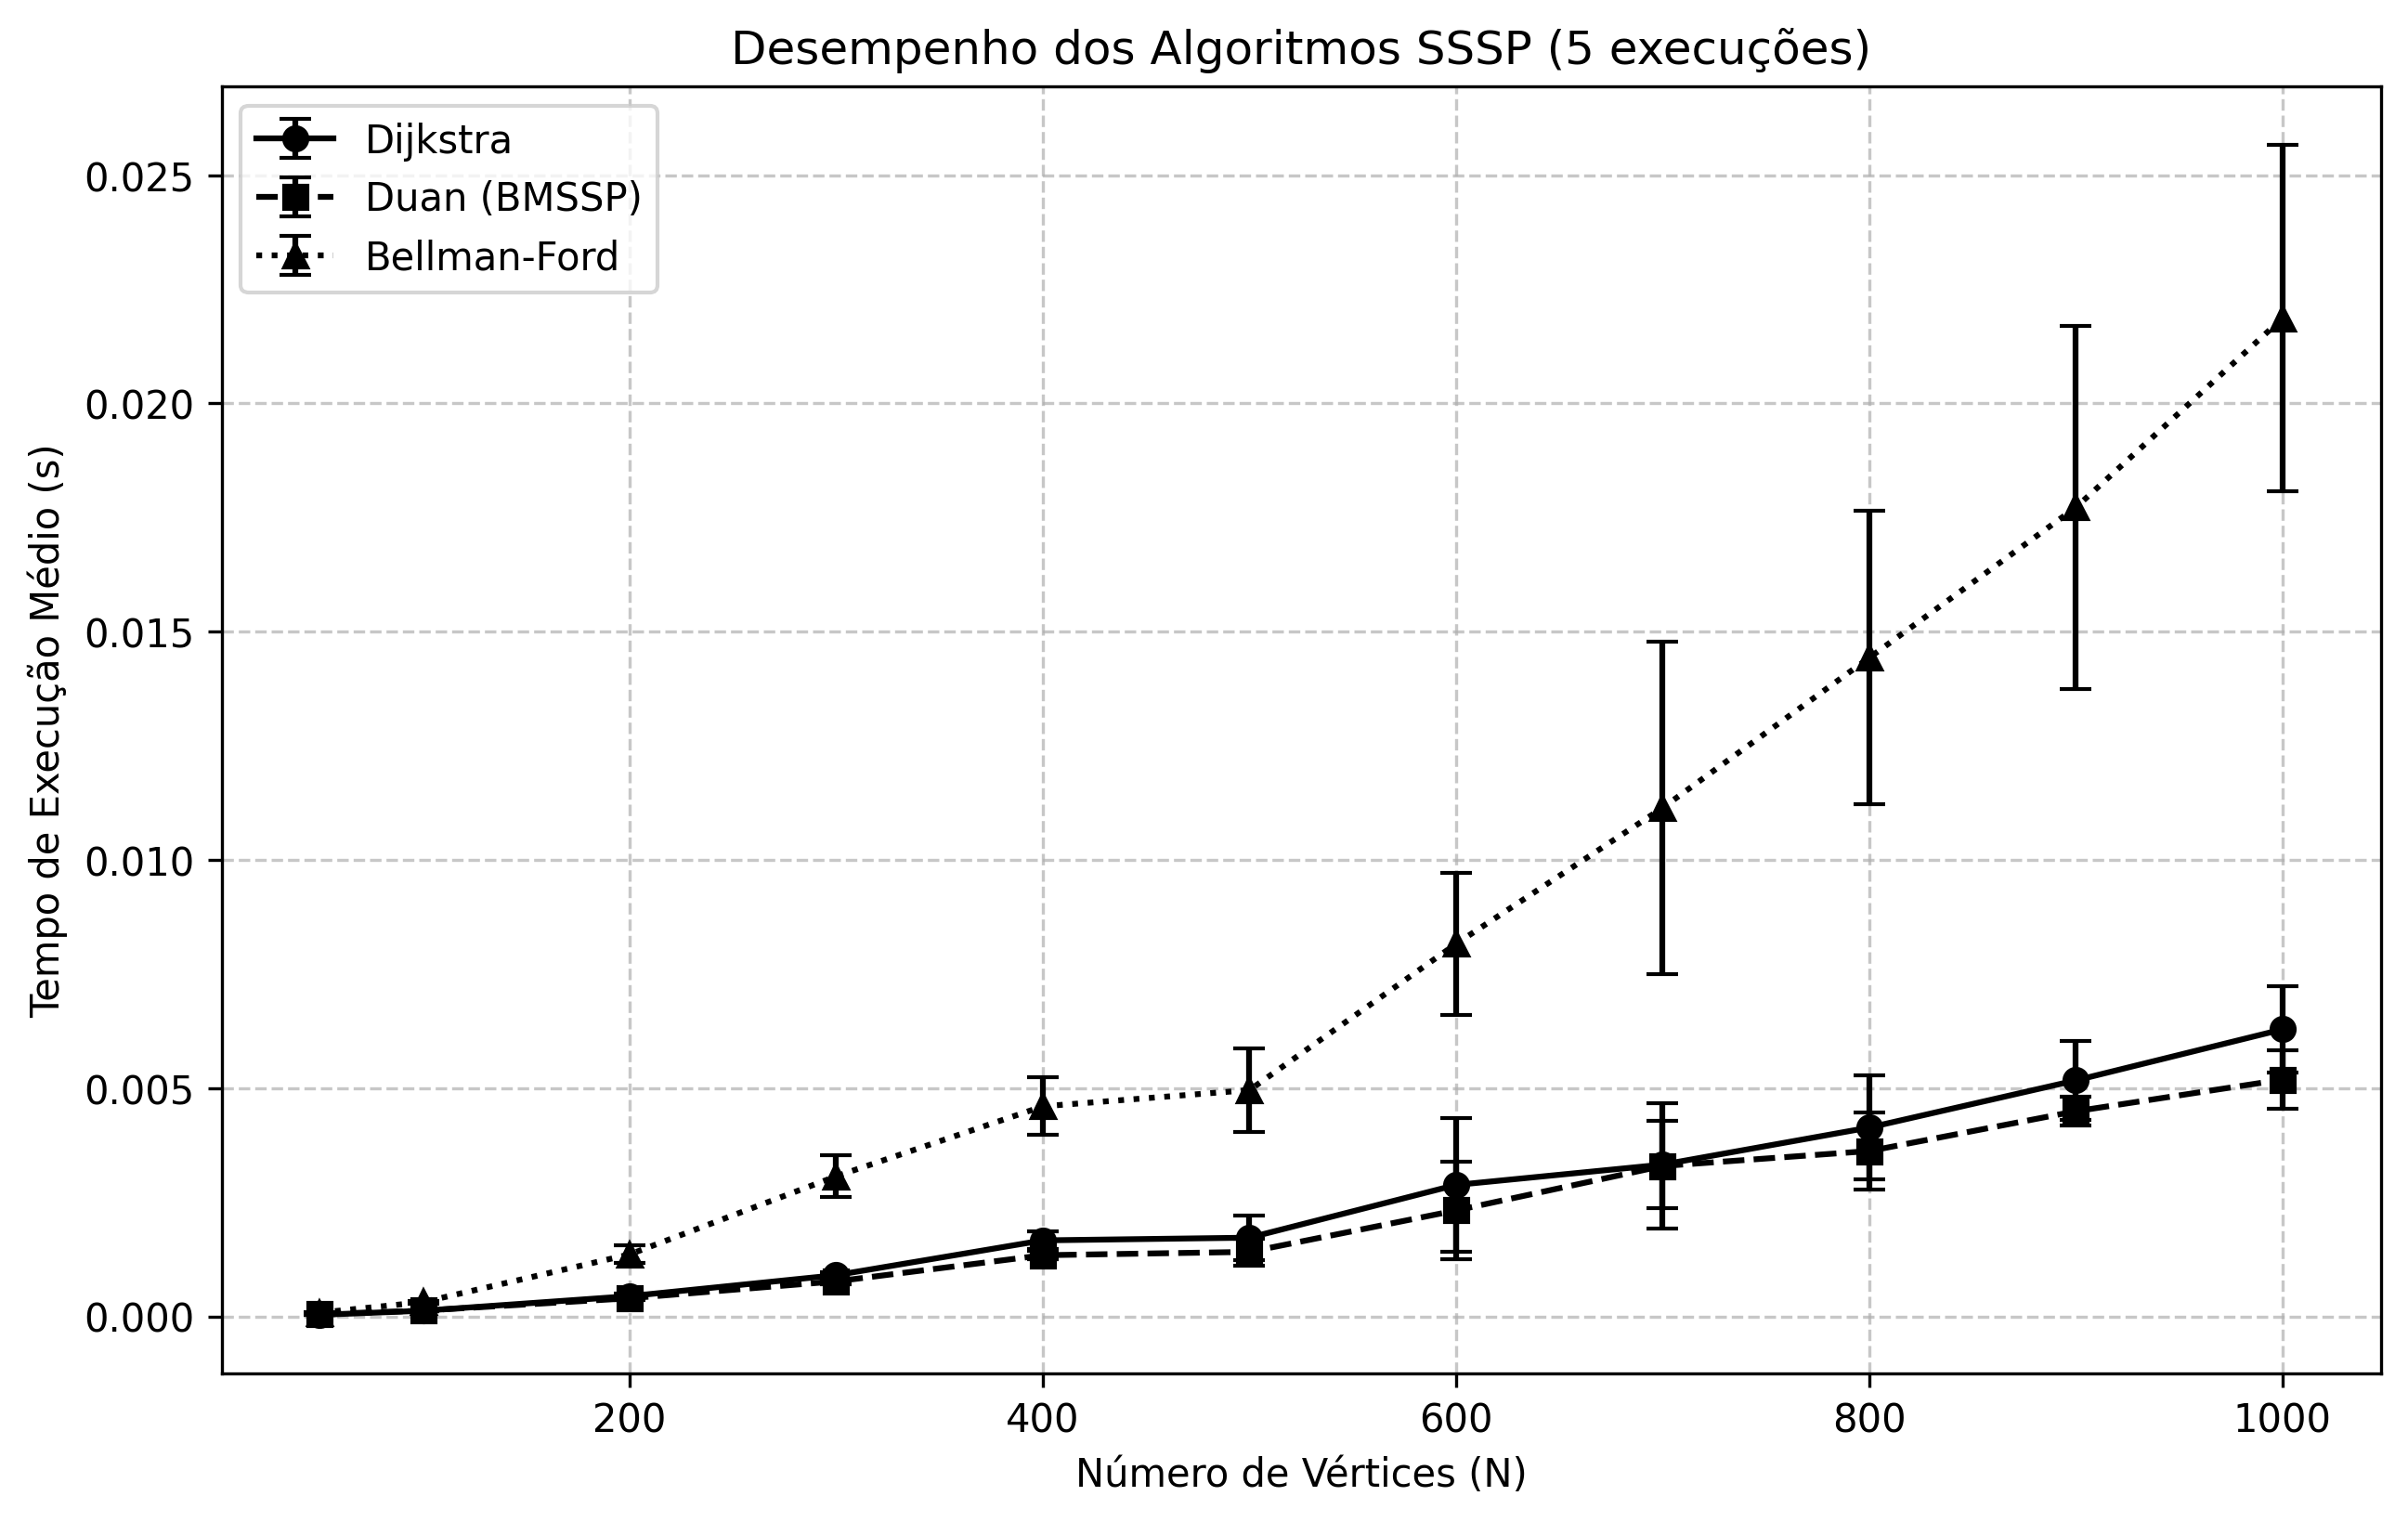
\includegraphics[width=0.65\textwidth]{../relatorio_tp03/desempenho_algoritmos_pb.png}
    \end{center}
    \vspace{-0.3cm}
    \begin{itemize}
        \small
        \item \textbf{Dijkstra Clássico} (Min-Heap): Desempenho hiper-otimizado com constante estrutural quase nula.
        \item \textbf{BMSSP (Duan)}: Vantagem teórica penalizada pelo \textit{overhead} de chamadas recursivas, alocação de conjuntos e \texttt{FindPivots} em instâncias menores ($N \le 1000$).
        \item \textbf{Bellman-Ford (Baseline)}: Rápida explosão combinatória devido à validação exaustiva $\mathcal{O}(|V||E|)$.
    \end{itemize}
\end{frame}

\begin{frame}{Resultados Estatísticos (5 Execuções Independentes)}
    \begin{table}[htbp]
\centering
\caption{Tempo de Execução (média $\pm$ desvio padrão em segundos) para 5 execuções independentes.}
\label{tab:estatistica}
\resizebox{\textwidth}{!}{
\begin{tabular}{rccc}
\toprule
\textbf{Vértices ($N$)} & \textbf{Dijkstra} & \textbf{BMSSP (Duan)} & \textbf{Bellman-Ford (Outro)} \\
\midrule
50 & 0.0000 $\pm$ 0.0000 & 0.0001 $\pm$ 0.0000 & 0.0001 $\pm$ 0.0000 \\
100 & 0.0001 $\pm$ 0.0000 & 0.0001 $\pm$ 0.0000 & 0.0003 $\pm$ 0.0000 \\
200 & 0.0004 $\pm$ 0.0000 & 0.0004 $\pm$ 0.0000 & 0.0014 $\pm$ 0.0002 \\
300 & 0.0009 $\pm$ 0.0001 & 0.0008 $\pm$ 0.0001 & 0.0031 $\pm$ 0.0005 \\
400 & 0.0017 $\pm$ 0.0002 & 0.0013 $\pm$ 0.0001 & 0.0046 $\pm$ 0.0006 \\
500 & 0.0017 $\pm$ 0.0005 & 0.0014 $\pm$ 0.0003 & 0.0050 $\pm$ 0.0009 \\
600 & 0.0029 $\pm$ 0.0015 & 0.0023 $\pm$ 0.0011 & 0.0082 $\pm$ 0.0016 \\
700 & 0.0033 $\pm$ 0.0009 & 0.0033 $\pm$ 0.0014 & 0.0111 $\pm$ 0.0036 \\
800 & 0.0041 $\pm$ 0.0011 & 0.0036 $\pm$ 0.0008 & 0.0144 $\pm$ 0.0032 \\
900 & 0.0052 $\pm$ 0.0009 & 0.0045 $\pm$ 0.0003 & 0.0177 $\pm$ 0.0040 \\
1000 & 0.0063 $\pm$ 0.0009 & 0.0052 $\pm$ 0.0006 & 0.0219 $\pm$ 0.0038 \\
\bottomrule
\end{tabular}
}
\end{table}

\end{frame}

% ==============================================================================
\section{Conclusões}
% ==============================================================================
\begin{frame}{Considerações Finais}
    \begin{itemize}
        \item O ganho assintótico teórico do BMSSP ($O(m \log^{2/3} n)$) é um feito matemático excepcional (Duan et al.).
        \item Contudo, observamos no experimento (via Profiling) que o tempo prático é severamente influenciado pelas chamadas recursivas, alocação excessiva da matriz e operações de amostragem.
        \item O \textbf{Dijkstra Clássico} aliado a um Min-Heap nativo com manipulação eficiente de ponteiros exibe \textit{overhead} prático tão baixo que costuma vencer em tempo real no hardware moderno em cenários sub-quadráticos.
        \item O ambiente de CI/CD via \texttt{Makefile} permite rápida replicação, colaboração inter-equipes fluida e geração determinística da documentação científica.
    \end{itemize}
\end{frame}

\begin{frame}
    \centering
    \Huge \textbf{Obrigado!} \\
    \vspace{1cm}
    \Large Dúvidas?
\end{frame}

\end{document}
